\section{Experimental Validation}\label{sec:SimResults}
The proposed SINF framework is validated on a high-fidelity core loss dataset $\mathcal{D}=\{(f_i, B_i, P_{v,i})\}_{i=1}^{N}$ measured on Fair-Rite~95 at $25\,^{\circ}$C by a parallel-resonance-based automated measurement system \cite{11121265} shown in Fig.~\ref{fig:data}(a). The dataset contains $N=1320$ sinusoidal operating points covering a wide range of frequency, peak flux density and core loss, as shown in Fig.~\ref{fig:data}(b). The points are split into a $80\%$ training set of $1056$ samples and a $20\%$ test set of $264$ sample. All variables are normalized by their training means $f_{n}=372.6$~kHz, $B_{n}=102.6$~mT, and $P_{v,n}=303.9$~mW/cm$^{3}$, so that the identified coefficients are of comparable order. The framework is implemented in PyTorch and the hyperparameters are listed in Table~\ref{tab:hyper}.


\begin{table}[t]
\centering
\caption{Predefined Hyperparameters for SSI Training}
\vspace{-8pt}
\label{tab:hyper}
\small
\begin{tabular}{cccccccc}
\toprule
\rowcolor{gray!15}
\textbf{Parameter} & \textbf{Value} & \textbf{Parameter} & \textbf{Value} & \textbf{Parameter} & \textbf{Value} & \textbf{Parameter} & \textbf{Value}\\
\midrule
Library size $M$   & 103   & Sample Size $N$ & 1320  & Log weight $w_{1}$  & 0.5  & MAPE weight $w_{2}$  & 0.5   \\
Learning rate $\eta$ & $0.005$  & Weight decay $\gamma$  & 0.05  & Threshold $\lambda_{\max}$ & 0.1 &  Constant $\epsilon$  & $10^{-8}$   \\
\bottomrule
\end{tabular}
\end{table}

The training history is shown in Fig.~\ref{fig:results}. The objective in Fig.~\ref{fig:results}(a) falls steeply at first and converges as the coefficients are completely refined. Fig.~\ref{fig:results}(b) shows the history of the active terms in the library, finally reaching $7$ terms and remaining unchanged. Fig.~\ref{fig:results}(c) illustrates how the coefficients evolve, where only active coefficients converge to steady values while others are pruned as zero. 

\begin{figure}[t] 
    \centering
    \vspace{-5pt}
    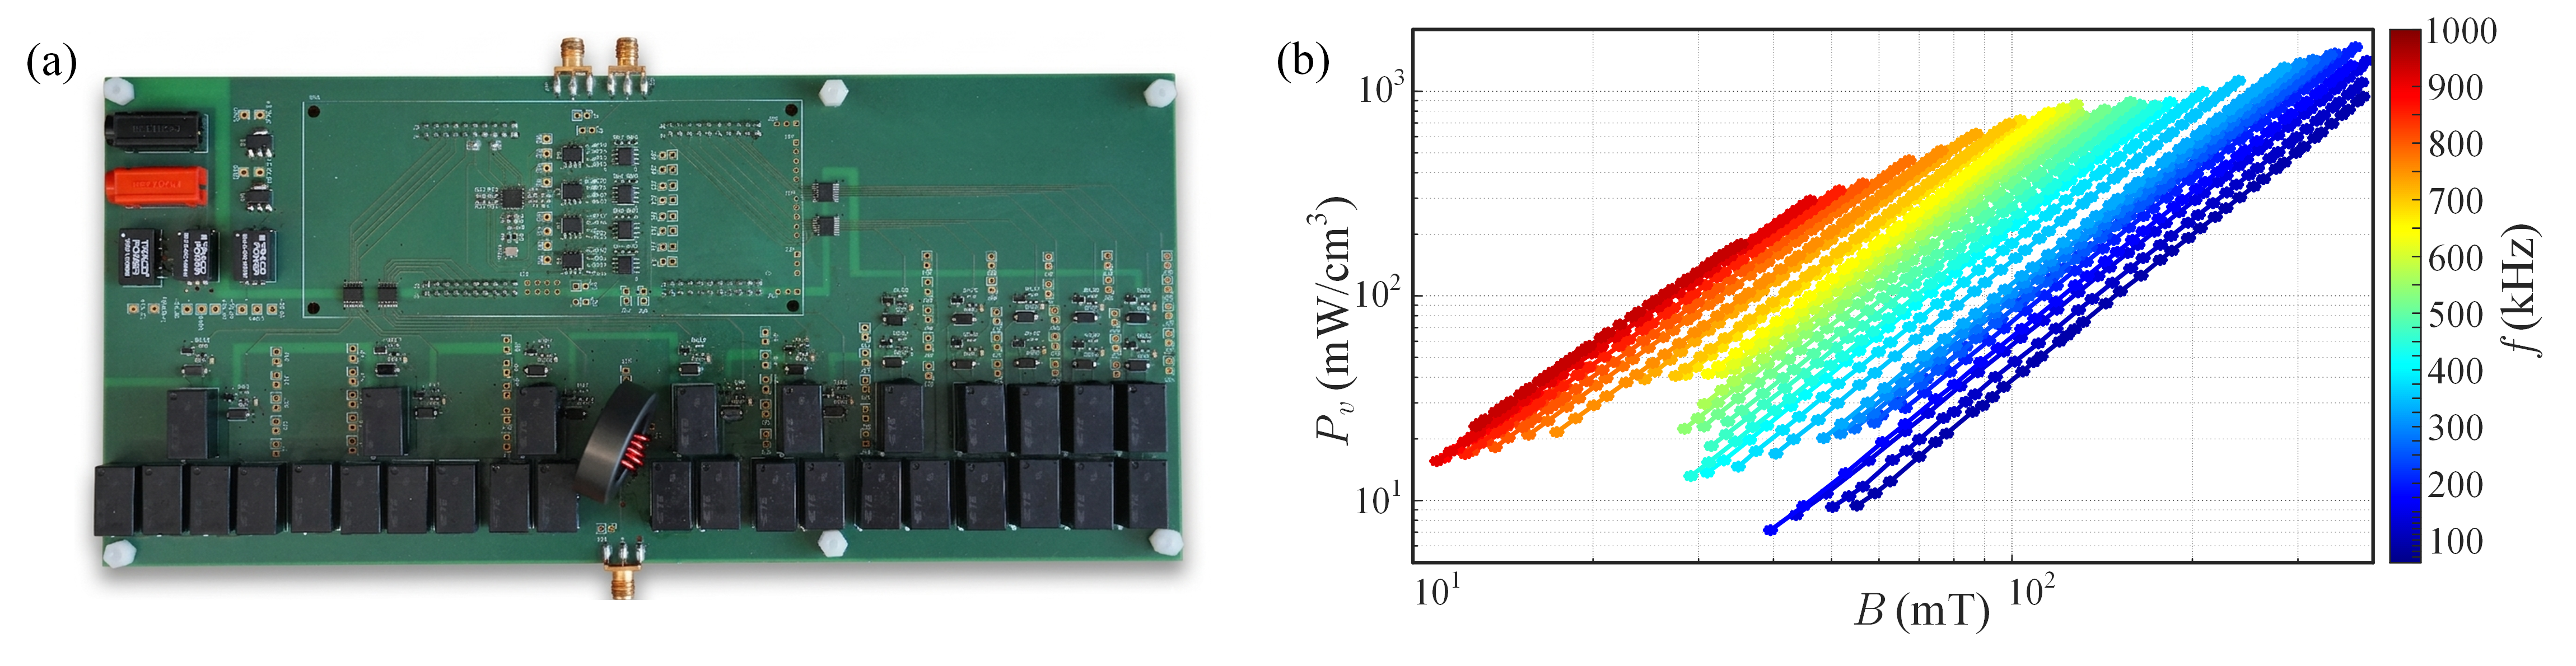
\includegraphics[width=0.95\textwidth]{Figure2.png} 
    \vspace{-10pt}
    \caption{(a) The automated measurement system. (b) High-fidelity dataset of Fair-Rite 95 collected by the system.}
    \label{fig:data}
\end{figure}

\begin{figure}[t] 
    \centering
    \vspace{-5pt}
    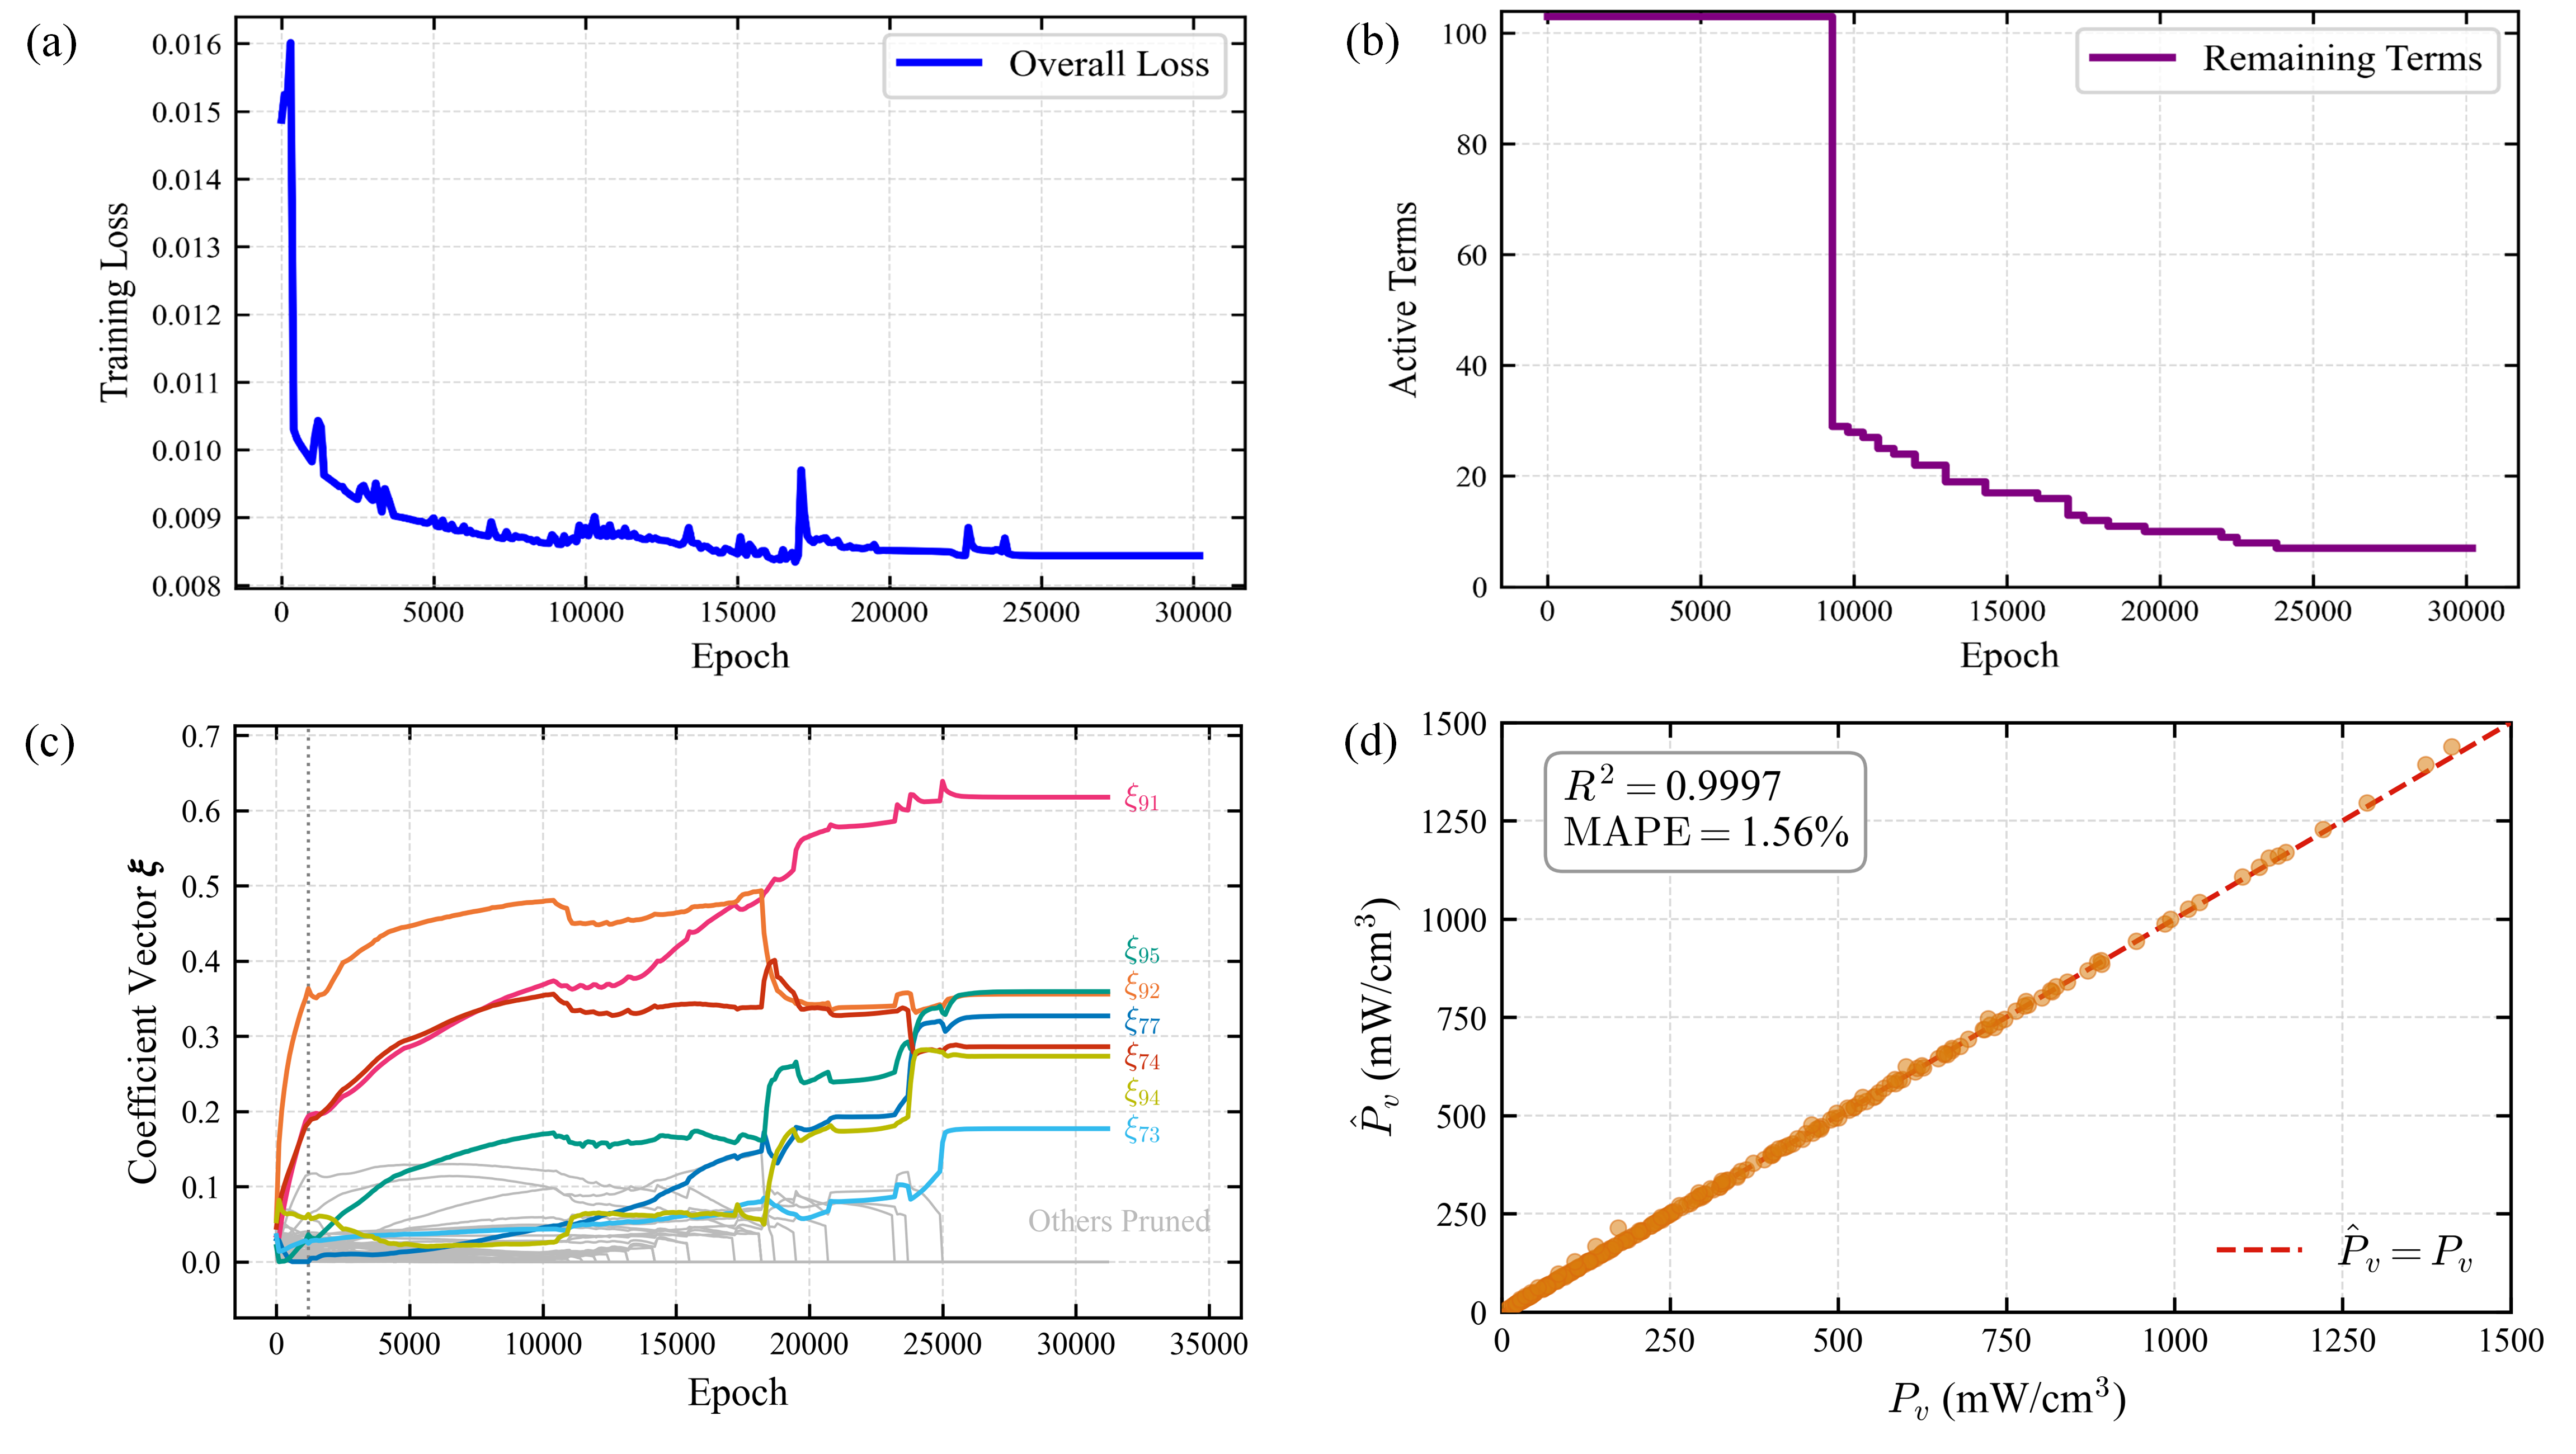
\includegraphics[width=0.95\textwidth]{Figure3.png} 
    \vspace{-10pt}
    \caption{(a) The history of the training loss. (b) The history of the remaining active terms. (c) The history of the evolving coefficients. (d) The pareto comparison between the discovered model and measured data.}
    \label{fig:results}
\end{figure}


\begin{table}[t]
\centering
\caption{Identified Parameters of the Discovered Core Loss Model}
\vspace{-8pt}
\label{tab:params}
\small
\begin{tabular}{lccccccccccccc}
\toprule
\textbf{Symbol} & $\xi_{91}$ & $\xi_{77}$ & $\xi_{74}$ & $\xi_{92}$ & $\xi_{94}$ & $\xi_{95}$ & $\xi_{73}$ &  $\alpha_{91}$ &  $\alpha_{77}$ &  $\alpha_{74}$ &  $\bar{f}_{c,91}$ & $\bar{f}_{c,77}$ & $\bar{f}_{c,74}$ \\
\midrule
\textbf{Value}  & $1.2729$  & $0.4735$  & $0.4819$  & $0.4591$  & $0.3981$  & $0.4054$  & $0.2984$  & $2$ & $1$ & $1$ & $3.00$ & $0.75$ & $0.50$ \\
\bottomrule
\end{tabular}
\end{table}


The discovered equation retains $7$ of $103$ candidates and takes the explicit form: 
\vspace{-10pt}
\begin{equation}
\begin{aligned}
\bar{P}_v =
\underbrace{\sum_{j=91,77,74}
\frac{\xi_{j}\,\bar{f}^{\,\alpha_{j}}\bar{B}^{2}}
{1+\big(\bar{f}/\bar{f}_{c,j}\big)^{2}}}_{\text{eddy-current with HF roll-off}}
\;+\;
\underbrace{\xi_{92}\,\bar{f}\bar{B}^{2}\ln\bar{B}
+\xi_{94}\,\bar{f}^{1.4}\bar{B}^{2.4}\ln\bar{B}
+\xi_{95}\,\bar{f}^{1.4}\bar{B}^{2.4}\ln\bar{f}}_{\text{Steinmetz-exponent drift}}
\;+\;
\underbrace{\xi_{73}\,\bar{f}^{1.5}\bar{B}^{1.5}}_{\text{excess}} 
\end{aligned}
\label{eq:discovered}
\end{equation}
where $\bar{f}=f/f_{n}$, $\bar{B}=B/B_{n}$, $\bar{P}_v=P_v/P_{v,n}$. The identified coefficients and their corresponding parameters are listed in Table~\ref{tab:params}. Fig.~\ref{fig:results}(d) compares the predicted and measured loss on the test set, where the points lie on the $\hat{P}_v=P_v$ diagonal across the full range. The discovered equation attains $R^{2}=0.9997$ and $\mathrm{MAPE}=1.56\%$ on the test set. Note that the accuracy can potentially be further improved with a smaller resolution of the exponent grid, which requires an extension of candidate library.  

\begin{table}[t!]
\centering
\caption{Comparison of State-of-the-art Modeling Methods.}
\vspace{-5pt}
\label{tab:metrics}
\renewcommand{\arraystretch}{1.3}
\begin{tabular}{lcccc}
\toprule
\rowcolor{gray!15}
Modeling Methods & SE & Random Forest & Feedforward Neural Network & \textbf{Proposed SINF}\\
\midrule
MAPE         & $10.92\%$ & $5.13\%$ & $1.37\%$ & $\mathbf{1.56\%}$  \\
$R^2$ Score  & $0.9868$  & $0.9961$ & $0.9996$ & $\mathbf{0.9997}$  \\
Parameter Number   & $3$       & $199{,}555$ & $4417$ & $\mathbf{7/103}$  \\
Active Terms & $1$       & Black Box & Black Box & $\mathbf{7/103}$  \\
\bottomrule
\end{tabular}
\end{table}

The proposed SINF is compared against the empirical SE, a random forest regressor and a feedforward neural network to verify its superiority. The quantitative results are summarized in Table~\ref{tab:metrics}. Note that SINF obtaining great accuracy and condenses the analytical equation with only $7$ active terms, thus achieving significant improvement against the SE and other data-driven methods.

% The recovered structure is physically
% interpretable. The first group reproduces the classical $f^{2}B^{2}$
% eddy-current dependence but attenuates it above a set of cutoffs,
% which accounts for the non-monotone apparent Steinmetz exponent measured
% on this dataset ($\alpha=1.27$, $1.58$ and $1.44$ over the lower,
% middle and upper frequency thirds). The logarithmic group is the
% first-order expansion of an exponent that drifts with excitation level,
% and it captures the measured variation of $\beta$ from $2.48$ at low
% frequency to $2.14$ at high frequency, which no fixed-exponent power law
% can represent. The excess-loss term recovers the $f^{1.5}B^{1.5}$
% scaling of anomalous loss without it having been imposed.

% Fig.~\ref{fig:parity} compares the predicted and measured loss on the
% held-out test set. The discovered equation attains $R^{2}=0.9997$ and
% $\mathrm{MAPE}=1.56\,\%$ on the test set against $1.58\,\%$ on the
% training set; the absence of a train-test gap indicates that a
% seven-term model selected from $103$ candidates does not overfit
% $1056$ samples. The residual distributions in Fig.~\ref{fig:residuals}
% are centered and near-symmetric, and the scatter against $f$ and $B$ in
% Fig.~\ref{fig:scatter} shows no systematic trend across the operating
% plane, indicating that the retained library spans the dominant loss
% mechanisms rather than absorbing them into a biased fit.

% Table~\ref{tab:compare} compares SSI against the classical SE and
% against an SE extended with second-order logarithmic corrections, both
% fitted on the identical training split. The SE reduces the test error to
% $10.65\,\%$ at best, which is the accuracy ceiling imposed by its fixed
% three-parameter structure; the extended variant improves this to
% $3.45\,\%$ but requires the correction terms to be postulated in
% advance. SSI reaches $1.56\,\%$ while selecting its own structure from
% data, a $6.8\times$ error reduction over the SE at comparable
% expression complexity.

